\documentclass[../main/report.tex]{subfiles}
\begin{document}

\chapter{GPU}

The GPU is at the heart of the Demolicious system.
Inspired by SIMD and SIMT architecture and programming models, the GPU architecture is named 'GhettoCUDA' in honor of NVIDIAs CUDA environment.\todo{cite this}

The GhettoCUDA architecture is highly parallel, in that it allows for a great number of threads to execute in parallel on multiple streaming processors.
A thread is the unit of execution, in essence a single procedure, that when correctly parameterized by run-time values allows for the transformation of a set of input data to a graphical representation to be visualized by the HDMI module.
A simple kernel, requiring no input, might be one that for each pixel in the framebuffer stores the color red.

The main design challenge in creating a GPU-inspired system is managing to saturate the memory bus as much as possible, changing memory access patterns from clustering together in time to a more spread-out pattern.
To facilitate this, the architecture allowing for multiple threads to execute on each streaming processor core, with a staggered start.
This design decision allows for a steady stream of load/store instructions without requiring a system stall as one waits for memory requests to return.

\section{Responsibilities}

The GPU has a relatively simple job:
\begin{enumerate}
  \item
    Receive instructions and constant data from the MCU
  \item
    Receive kernel invocations from the MCU
  \item
    Write results to external SRAM
  \item
    Assert the 'computation finished' signal to the MCU
\end{enumerate}

\section{Architecture Overview}
\begin{figure}[H]
\centering
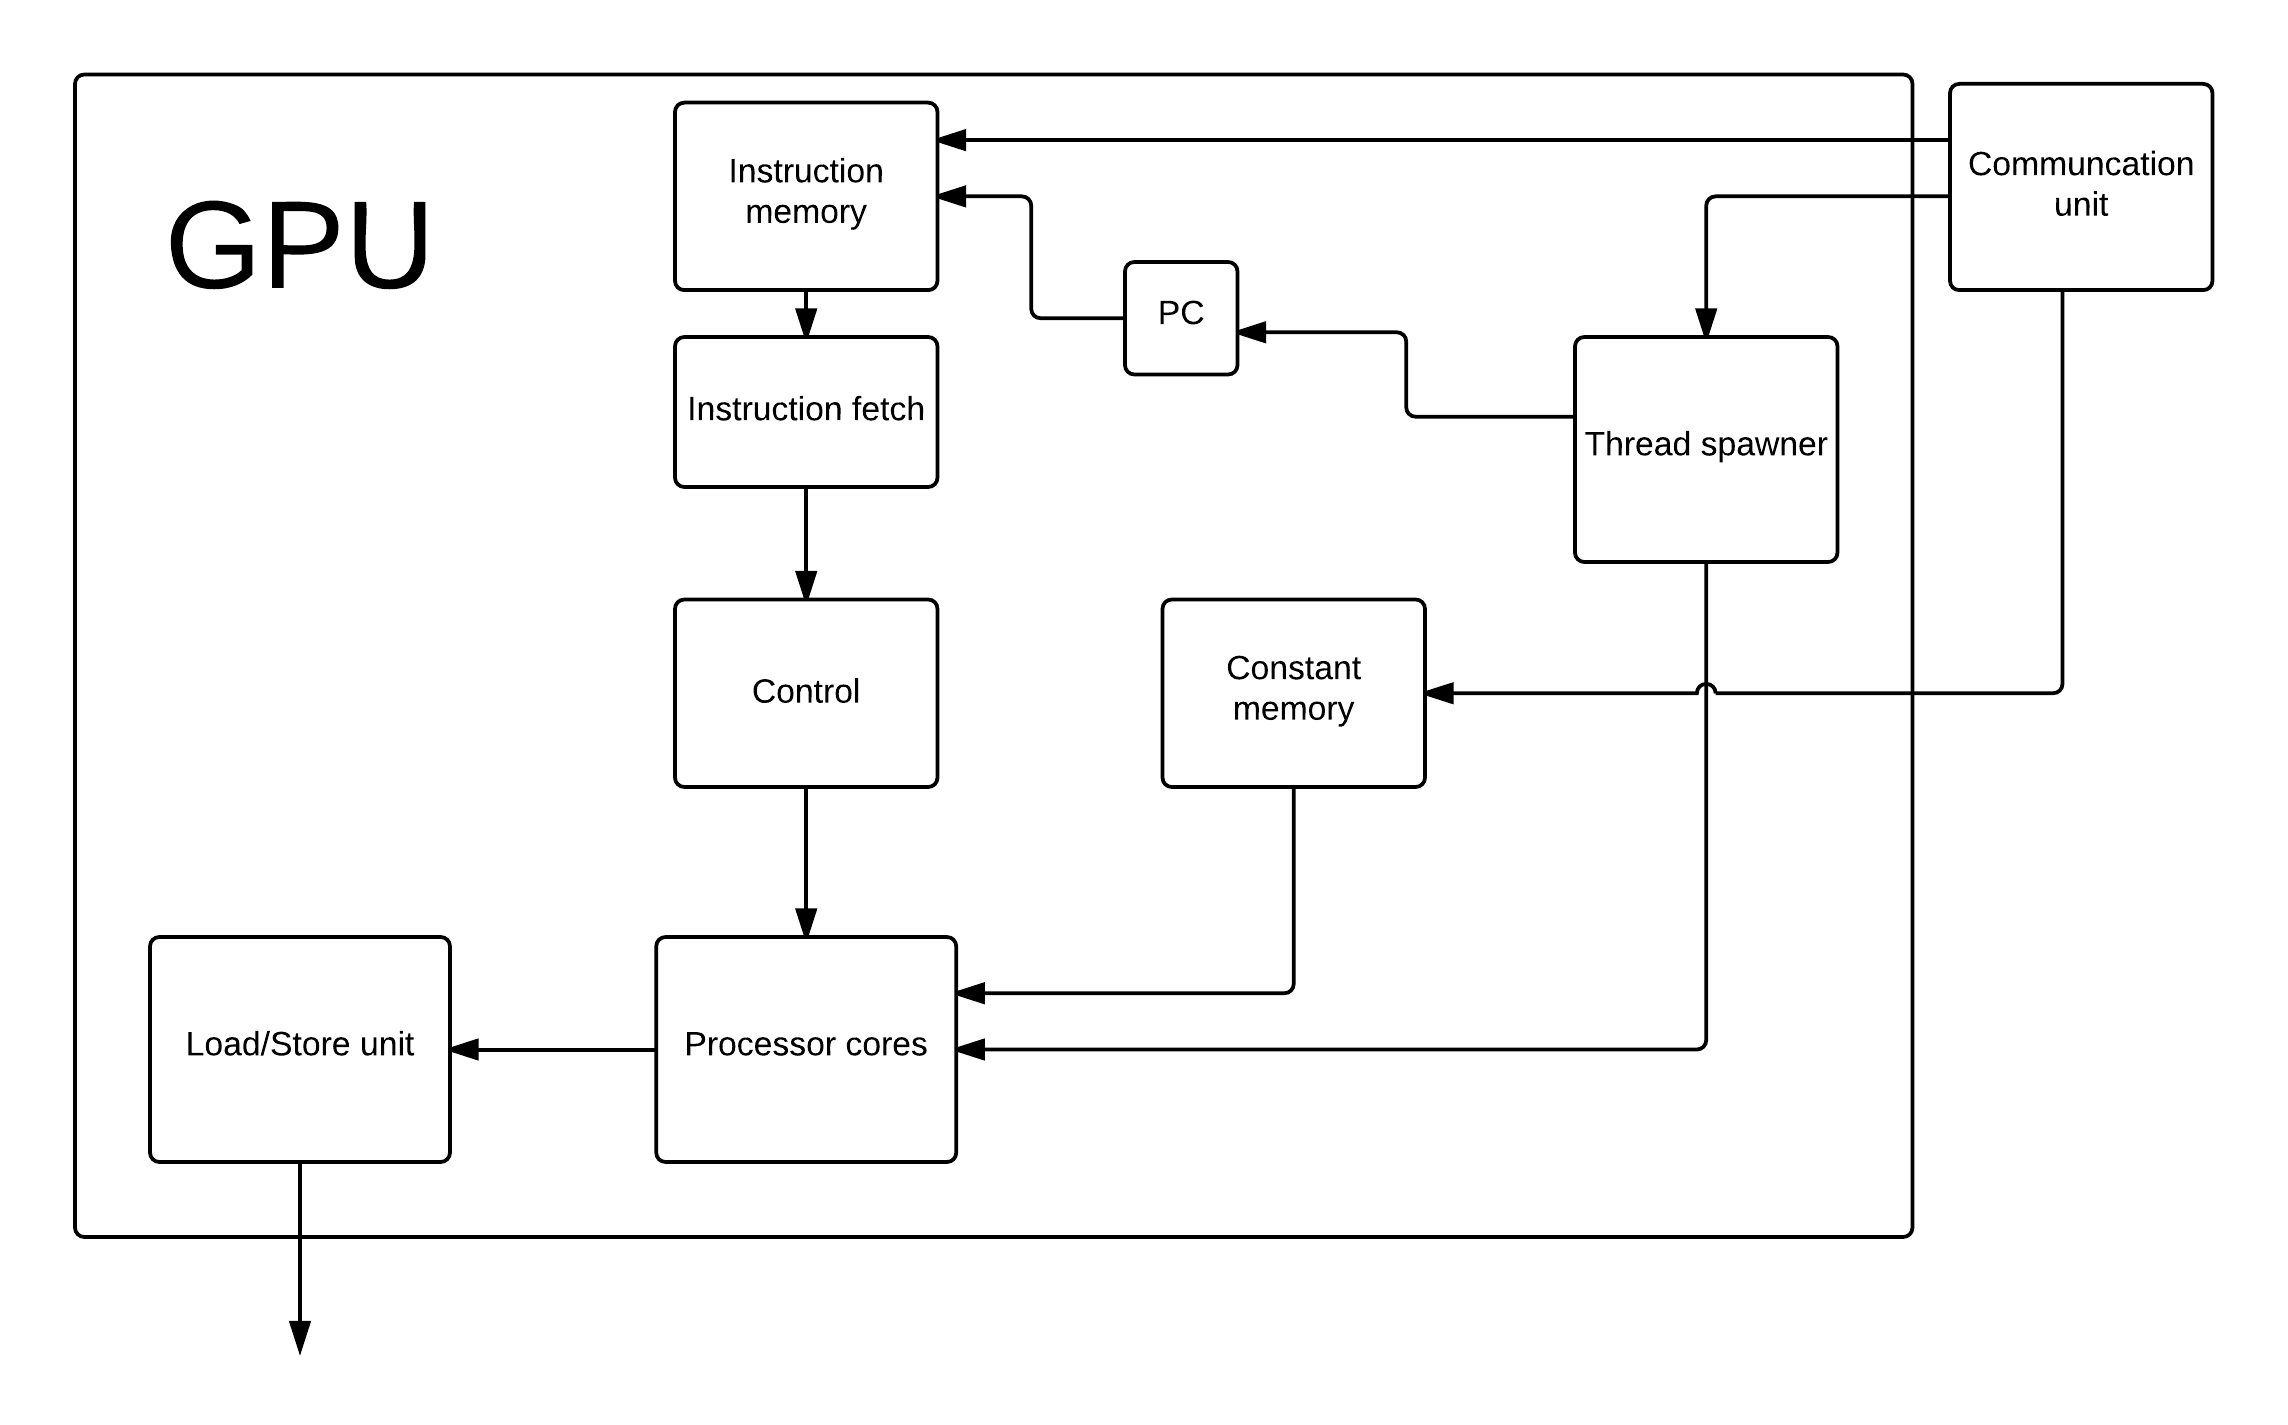
\includegraphics[width=\textwidth]{../gpu/diagrams/architecture_overview.png}
\caption{A high level overview of the GPU.}
\label{fig:architecture_overview}
\end{figure}
Figure \ref{fig:architecture_overview} presents a high level overview over the data-flow in the GPU.
The CPU issues commands to the GPU via the communication unit. Commands include actions such as launching a kernel, uploading kernels to the instruction memory, and writing to the constant memory.
Instructions are fetched from the instruction memory and decoded by the control unit, which has the responsibility of setting the control signals for the instructions.
The processors load constants from the constant memory, and uses the load/store unit for  accessing the data memory. 


\section{Kernel Structure}

\section{Receiving a Kernel Call}
\begin{figure}[H]
\centering
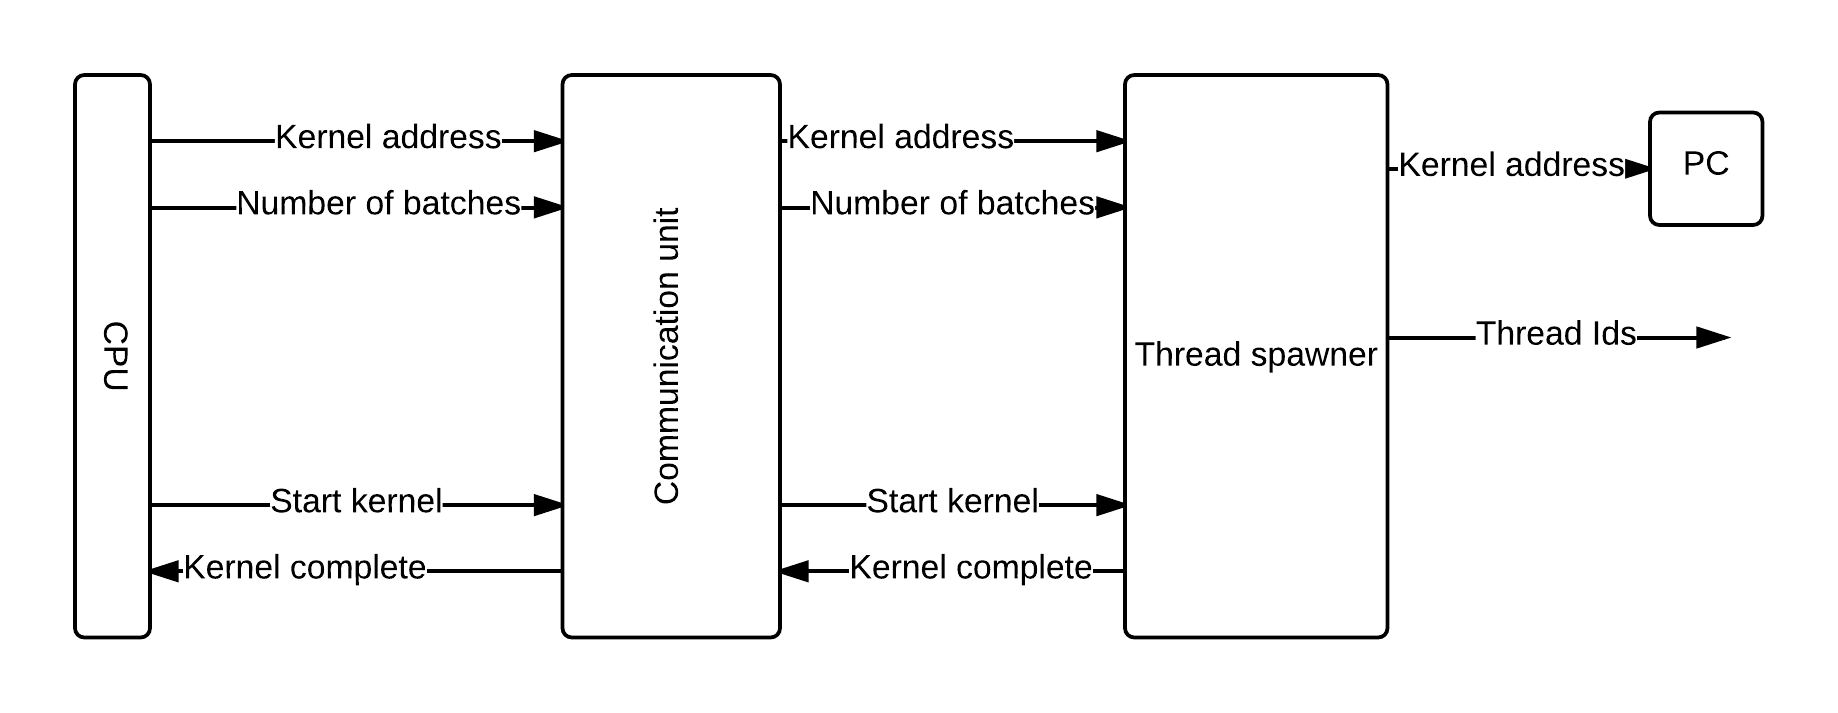
\includegraphics[width=\textwidth]{../gpu/diagrams/receiving_a_kernel_call.png}
\caption{Launching a kernel from the GPU's viewpoint.}
\label{fig:kernel_call}
\end{figure}

The communication unit is responsible for receiving kernel call requests from the CPU, and initiating the request.
A valid kernel call consists of the address of the kernel, the number of batches to launch, and asserting the launch signal.

The kernel launch signals are forwarded to the thread spawner, which writes the kernel start address to the PC register, and starts distributing threadIDs to the streaming processors. 
After holding the kernel launch signals high for one clock cycle, the communication unit has completed its role in launching the kernel.
When the kernel completes executing, the thread spawner asserts the kernel done signal, and the communication unit forwards the signal to the CPU, indicating that the kernel call has completed.


\section{Running a Kernel}
Once the thread spawner has been initiated by the communication unit, the kernel runs to completion without intervention by the CPU. 
At the beginning of a kernel run, the thread spawner assigns threadIDs to each warp in the barrel.
After the initial IDs have been assigned the GPU enters normal execution.
\begin{figure}[H]
	\centering
	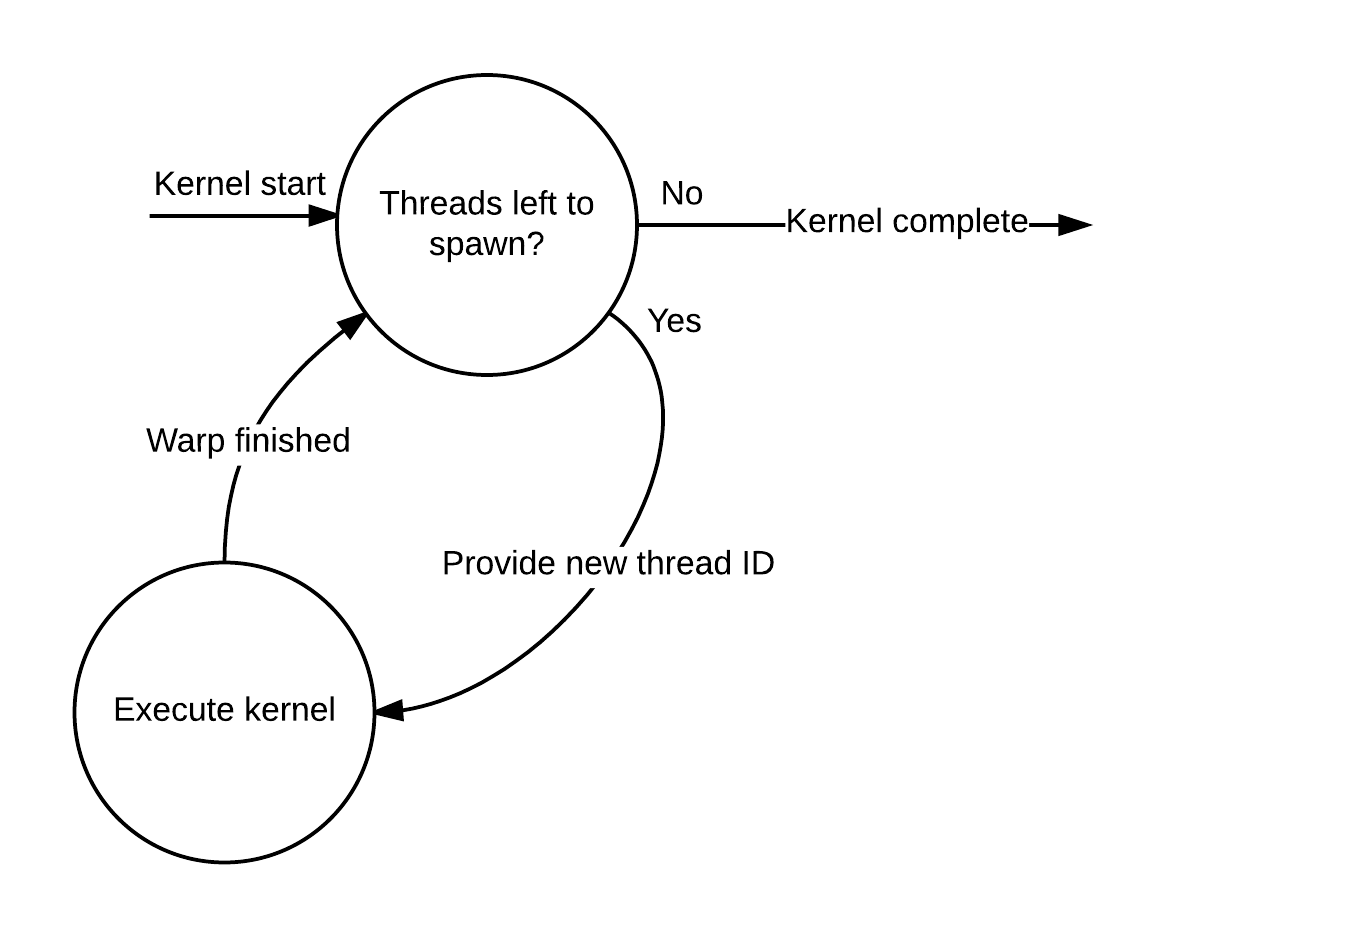
\includegraphics[width=0.9\textwidth]{../gpu/diagrams/kernel_run_state_machine.png}
	\caption{The GPU's internal state during kernel execution.}
	\label{fig:kernel_run_state_machine}
\end{figure}
A normal kernel execution can be represented by the state machine in figure \ref{fig:kernel_run_state_machine}.
During the kernel execution stage the warps execute the same instructions in lock-step one warp at a time, until the control unit encounters a \textit{Finished} instruction.
Upon receiving a \textit{Finished} instruction the control unit asserts the finished signal alerting the thread spawner that the warp requires new threadIDs.
The thread spawner keeps track of the number of threads awaiting launch.
When the thread spawner receives a \textit{Finished} instruction and no more threads are awaiting launch, the kernel run has completed.

\section{Component Details}

\todo{Can this be called something else? It's kind of confused with the component details in the PCB chapter}

\subsection{Streaming Processor}

The streaming processor is at the heart of the GhettoCUDA architecture.
A fully operational GhettoCUDA processor will have up to 32 streaming processors wired up, allowing for an extreme degree of parallelism in code execution.

The architecture of the streaming processor is inspired by the cores of the MIPS architecture.
They consist of a single ALU, a register bank, as well as logic for reading operands from thread-private registers, shared external memory and constant storage.
Each register bank is actually composed of several register files, containing a number of general- and special purpose registers.
The register bank mirrors the interface of the register file, but only exposes a single register file at a time, which one decided by the current active barrel line.
This system allows rapid context switching between the plethora of threads co-existing inside each streaming processor.

The streaming processor support conditional execution of instructions, using a dedicated mask register to decide whether instructions should be executed or not.
This allows for branch-like behavior without having to support the complex logic required for diverging threads.

When a memory request is invoked by the currently active instruction, memory addresses and data values are sampled from the currently active register file in the register directory, and passed on to the load/store unit.
Dedicated address and data store/return registers allows for simplification of both the programming model as well as requiring fewer wires between the set of streaming processors and the load/store unit.

\subsection{Thread Spawner}

The thread spawner is responsible for converting the MCUs request of n kernels executing kernel k on data set d to actual hardware threads.
As all kernels are uniquely identifiable by their respective thread ID, the thread spawner is responsible for providing strictly increasing and unique IDs.


\subsection{Register Directory}
\begin{figure}[H]
	\centering
	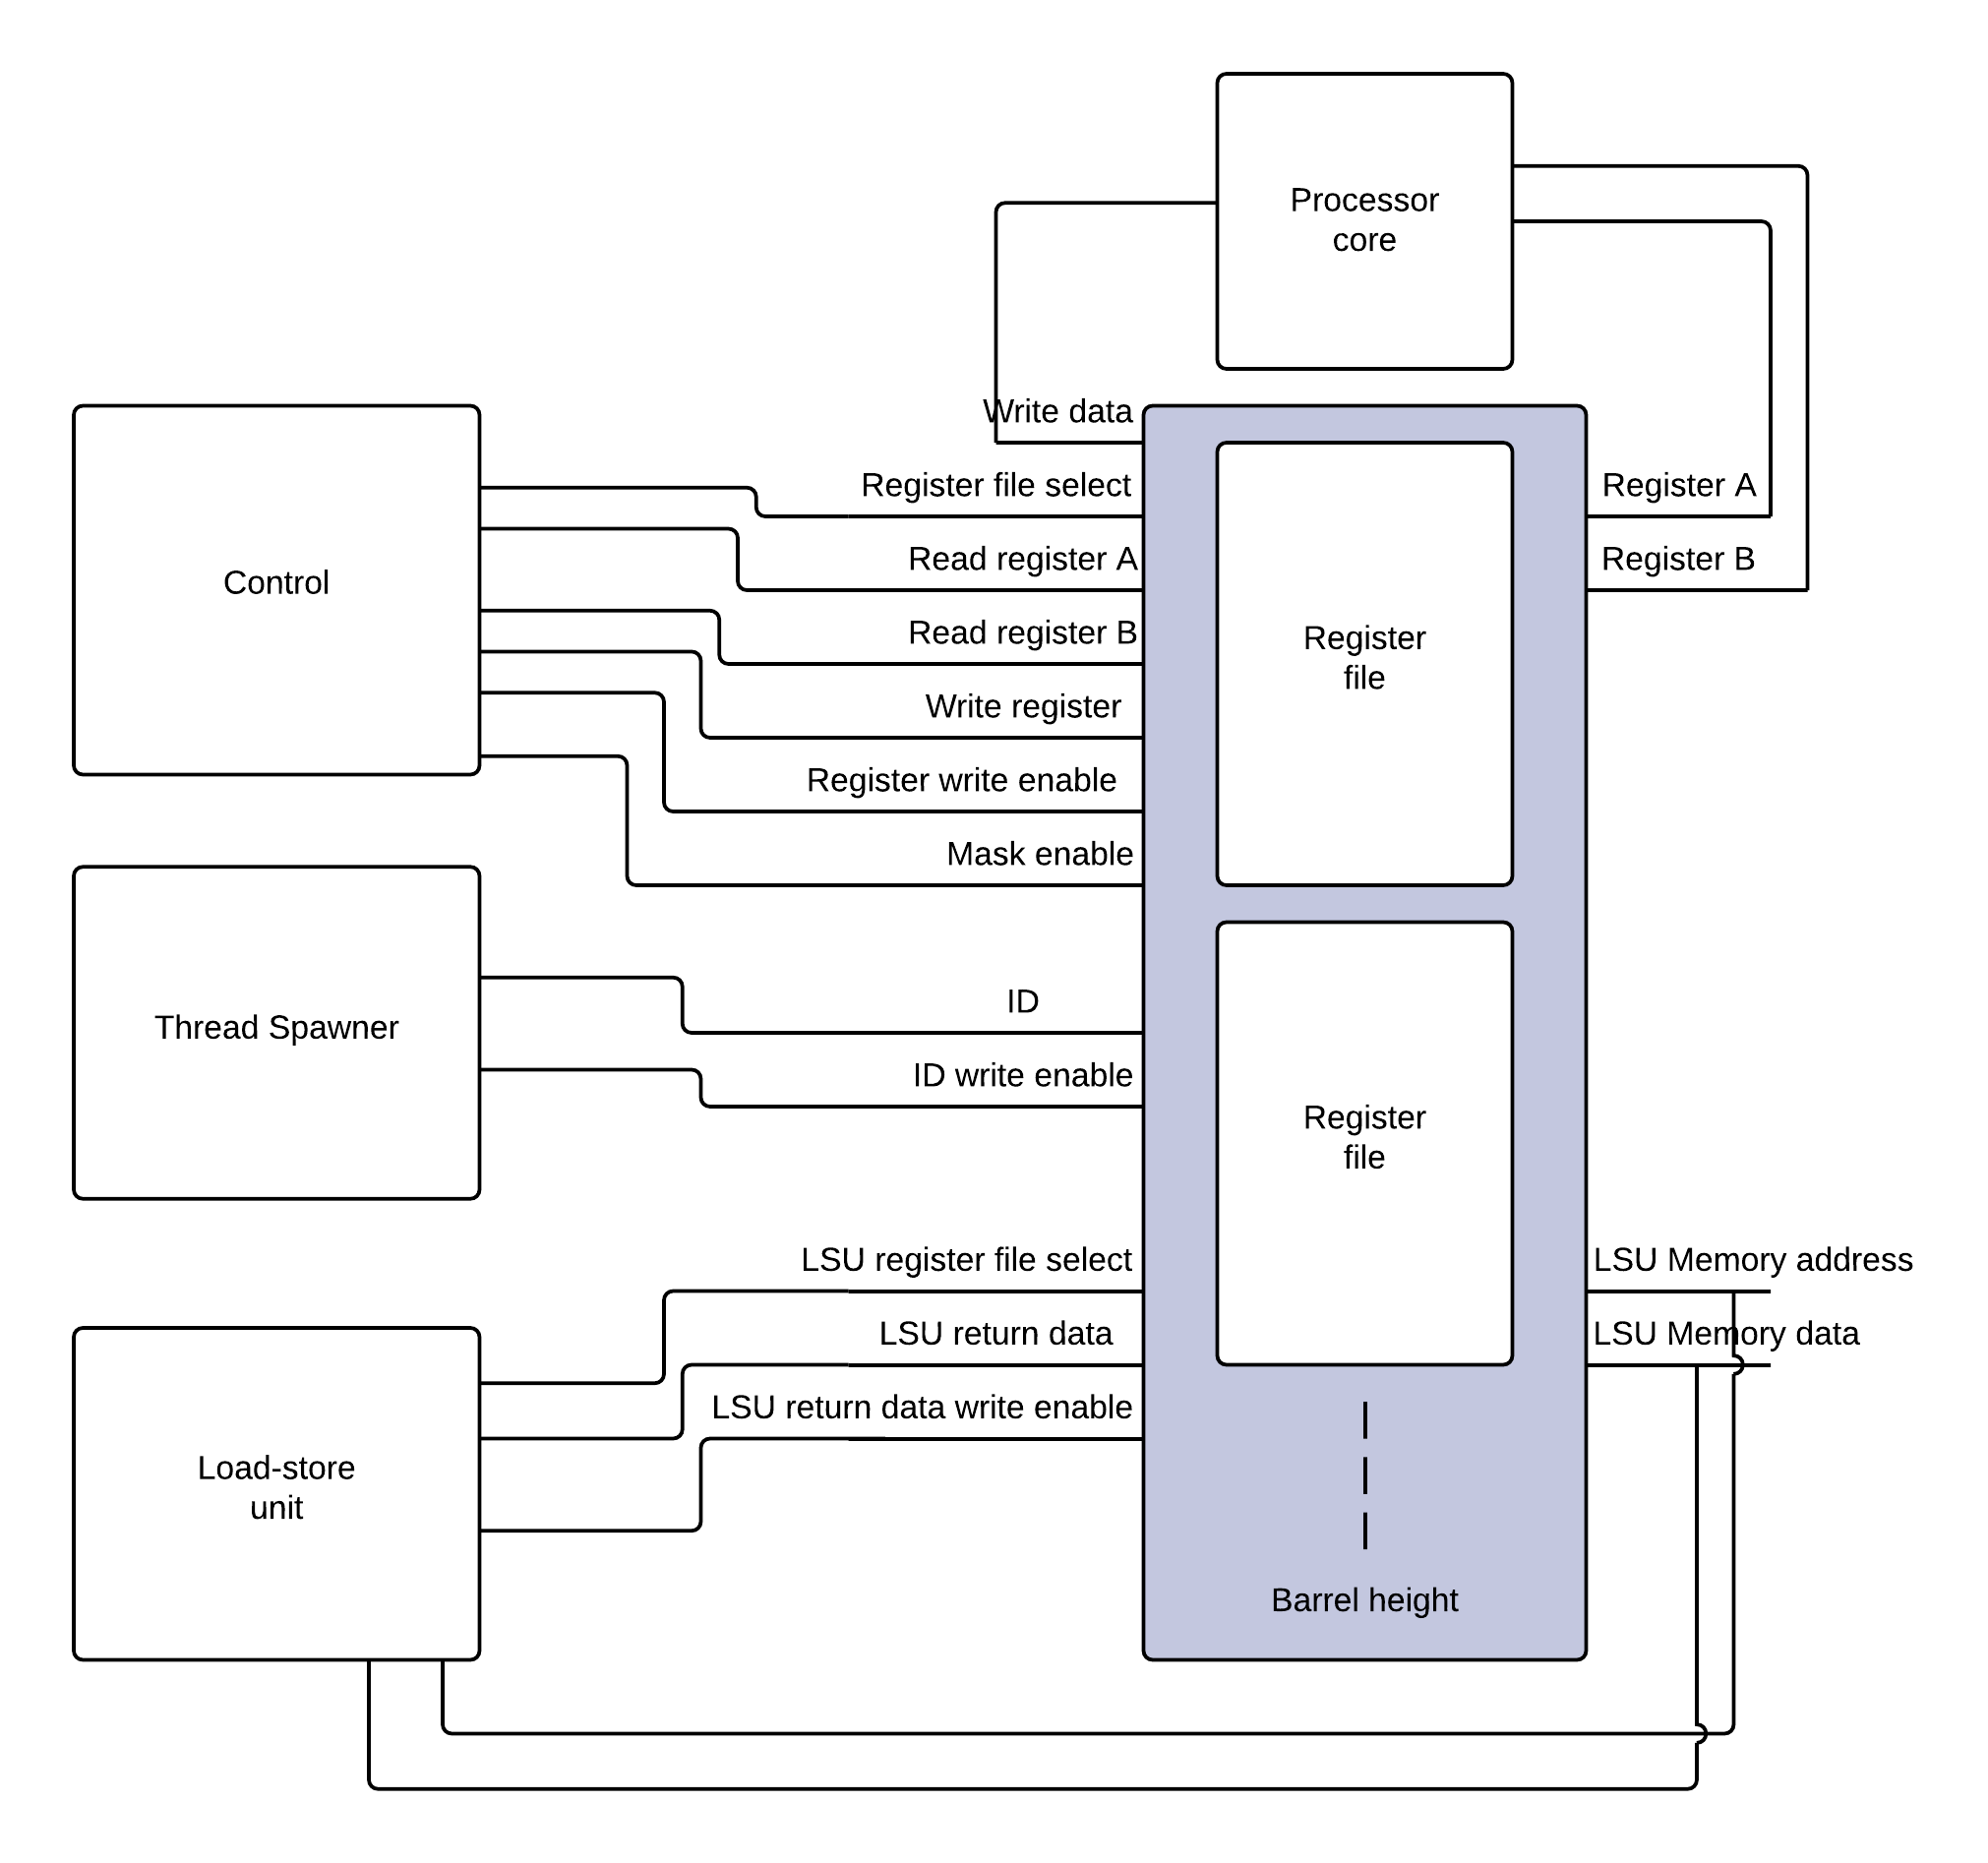
\includegraphics[width=\textwidth]{../gpu/diagrams/register_directory.png}
	\caption{The register directory, and its neighbouring components.}
	\label{fig:register_directory}
\end{figure}

There is one register directory per processor core.
Each register directory contains one register file per barrel row.
The register files include seven dedicated registers, and nine general purpose registers (Table \ref{tab:registers_overview}).

\begin{figure}[H]
	\centering
	\begin{tabular}{|c|c|c|}
		\hline Register number & Description & RW \\ 
		\hline \$0 & Zero register & Read-only \\ 
		\hline \$1 & ID High & Read/Write \\ 
		\hline \$2 & ID Low & Read/Write \\ 
		\hline \$3 & Address High & Read/Write \\ 
		\hline \$4 & Address Low & Read/Write \\ 
		\hline \$5 & LSU data & Read/Write \\ 
		\hline \$6 & Masking register & Write-only \\ 
		\hline \$7 - \$15 & General purpose registers & Read/Write \\ 
		\hline 
	\end{tabular} 
	\caption{The registers contained within the register files.}
	\label{tab:registers_overview}
\end{figure}

Individual register files are selected by using the \emph{register file select} signal.
The register file select signal is set by the control unit.
Within the register directory, the other input signals are routed to the selected register file using the select signal.
Consequently, from the processor core's point of view, there's just one register file.

The dedicated registers serve special purposes in the architecture.
Often, the processor core will be accessing a register file and at the same time, other components may also need access the same, or a different, register file.
To solve this, the special registers are given dedicated signals that the other components use for reading/writing to the register file.
Ignoring registers \$0 and \$6, the rest of the dedicated registers may be used as general purpose registers.
Using them at the same time as other components are accessing them will result in undefined behaviour, and is left as the programmer's responsibility.

The masking register is used to enable conditional execution.
If masking is enabled the first bit of masking register is used to disable writes to the register file, making the instruction have no effect (Figure \ref{fig:masking}).
\begin{figure}[H]
	\centering
	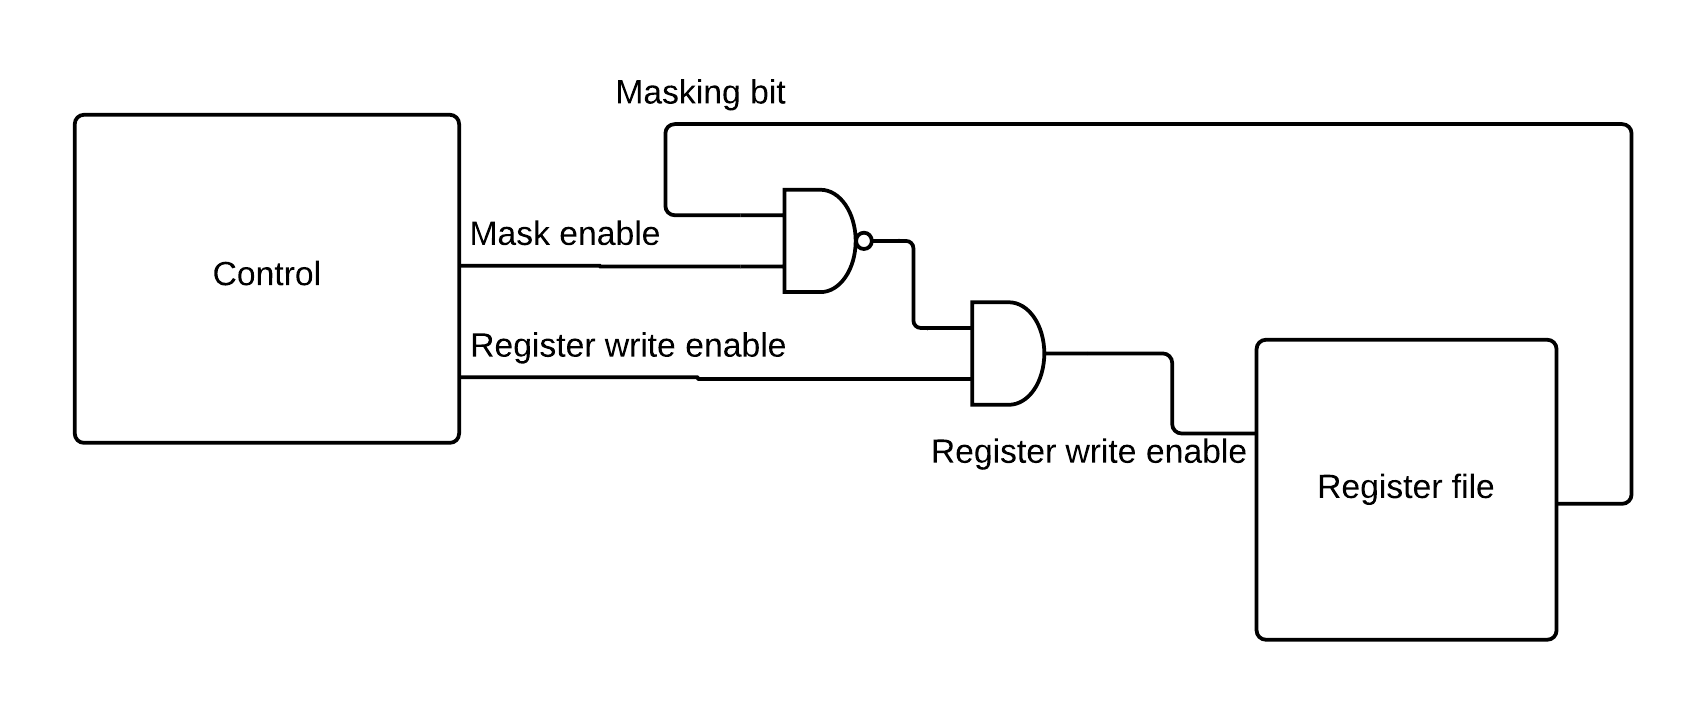
\includegraphics[width=0.8\textwidth]{../gpu/diagrams/masking.png}
	\caption{Using the mask bit to disable register writes.}
	\label{fig:masking}
\end{figure}

Data memory addresses are 20 bit wide, and thread IDs are 19 bit wide.
Registers can only store 16 bit values.	
To represent these values they are split into registers which contain the higher and lower bits.

The load store unit (LSU) has a separate signal for selecting register files.
Using the signal, the LSU can write data loaded from memory into the register files on its own.


\subsection{Load/Store Unit}
A load/store unit is responsible for handling memory requests from the core processors.
The load/store unit of Demolicious needs to be capable of simultaneously servicing incoming request from all the streaming processors.
Requests are asynchronously carried out in the background, and replies are delivered directly into the appropriate registers of the threads that made the request.

The peripheral design includes two independent memory banks, each capable of reading or writing one word every cycle.
To maximize the throughput to the memory, a word-striping scheme was used:
The lowest bit of the memory address determines which bank holds that location.

Because there are two independent memory banks, the incoming request are routed to two separate queues, one for each memory.
Each queue then feeds requests to its associated memory control unit.
Read responses are then handed to the write-back unit, which delivers the data to the appropriate register file.

The queues are necessary because Demolicious has more streaming processors than memory banks, so all the requests from a warp can not be completed in a single cycle.
The streaming processors work in tandem, and issue requests simultaneously.
Each memory bank can service at most one request per cycle.
As such, it takes several cycles to complete the requests for a single warp.
Since there is a limit to how many requests can be in the queue at any time, there is also a limit to how often requests can be issued.

\todo{The following does should be moved to another chapter.}
This several-cycle latency and queue size limit would have to be taken into consideration when programming for this architecture.
Loads would be not ready before several cycles later, and it would be ill-behaved to issue a request before there is room in the queue again.
To hide this latency a barrel is introduced to processor design.
A barrel makes the processor take turns executing warps from an active set in a round-robin fashion.
If the number of warps in a barrel is equal to the number of cycles of latency, the result of the first load of in the barrel can be used in the next instruction.

\end{document}
